\chapter{ \toolName の機能と外観}\label{cha:Function}
\toolName (Mix Visual Regression Test)は、レイアウトの不具合箇所の可視化を目的とした、視覚的回帰テストツールである。
本章では、本研究で試作したツール\toolName の機能と外観について説明する。
本研究で用いる「差分箇所」、「影響箇所」、「レイアウトの副作用箇所」、「レイアウトの不具合箇所」を、以下に定義する。
% 、「比較画像」、「比較HTMLコード」、「テスト画像」、「テストHTMLコード」
なお、\toolName は、「差分箇所」、「影響箇所」、「レイアウトの不具合箇所」の3つを強調する。
\begin{itemize}
    \item 差分箇所:\\
          変更前後のWebページの画像を比較して、
          変更前のWebページから削除された箇所と変更後のWebページに追加された箇所。
    \item 影響箇所:\\
          変更前後のWebページのHTMLコードを比較して、
          HTMLコードにおけるbody要素内の変更とstyle要素内の変更のどちらか、
          または両方の変更が適用された箇所。
    \item レイアウトの副作用箇所:\\
          変更前後のWebページの画像で、影響箇所によって、
          HTMLコードを変更していない画面要素にレイアウトの変更があった箇所。
    \item レイアウトの不具合箇所:\\
          レイアウトの副作用箇所のうち、画面要素の隠れ、見切れ、重なりがあった箇所。
          % \item 比較画像:\\
          %       視覚的回帰テストにおいて、比較対象とするWebページの画像。
          % \item 比較HTMLコード:\\
          %       視覚的回帰テストにおいて、比較対象とするWebページのHTMLコード。
          % \item テスト画像:\\
          %       視覚的回帰テストにおいて、テスト対象とするWebページの画像。
          % \item テストHTMLコード:\\
          %       視覚的回帰テストにおいて、テスト対象とするWebページのHTMLコード。      
\end{itemize}

\section{\toolName の機能}
\toolName は、WebページのURLを入力とする。
なお、入力対象とするWebページは、\ref{sec:target_images}節で述べた条件をすべて満たすものとする。
出力は、\ref{subsec:MixVRT_IO}節で後述する8つのPNG形式の画像を閲覧できるWebページである。
\par
開発者が\toolName を使用する際の流れを、以下に示す。
なお、\toolName を使用する想定として、開発者がWebページを作成しているとする。
\begin{enumerate}
    \item テキスト端末上で「\$ make test URL="WebページのURL"」を実行し、事前準備(\ref{subsec:MixVRT_preparation}節で後述)を行う。
    \item Webページの変更を行う。
    \item テキスト端末上で「\$ make test URL="WebページのURL"」を実行し、視覚的回帰テストを実行する。
    \item Webブラウザ上で「http://localhost:5000/MixVRT\_diff」にアクセスし、テスト結果を確認する。
    \item テスト結果を評価する
          \begin{itemize}
              \item 問題なし:「\$ make save」で変更前画像と変更前HTMLコードを更新する。
              \item 問題あり: 変更後のWebページを修正し、3に戻る。
          \end{itemize}
\end{enumerate}
以降、\toolName の機能について説明する。

\subsection{実行コマンド}\label{subsec:MixVRT_execution}
\toolName は、Python3.9.17\cite{Python}が動作するテキスト端末上で実行する。
\toolName 実行時のコマンドライン引数によって、視覚的回帰テストを行う入力対象のWebページのURLを指定する。
\toolName の実行コマンドの書式を、以下に示す。
\begin{lstlisting}[label=list:command,frame=none,numbers=none,basicstyle={\normalsize \ttfamily \color[gray]{.15}}]
  $ make test URL="WebページのURL"
 \end{lstlisting}
{\tt URL}には、入力対象とするWebページのURLを指定する。なお、WebページのURLは、"https://"または"http://"から始まるURLとする。
% また、初回実行時のみにおいて、{\tt URL}には、視覚的回帰テストを行うための比較対象とするWebページのURLを指定する。

% \toolName の初回実行時は、比較対象となるWebページの画像とHTMLコードが存在せず視覚的回帰テストを行えないため、
% 比較対象とするWebページのURLからWebページの画像とHTMLコードの取得のみを行い、処理を終了する。
% \toolName の2回目実行時は、テスト対象とするWebページのURLからWebページの画像とHTMLコードを取得し、
% 比較対象とするWebページの画像とHTMLコードに対して視覚的回帰テストを行う。
% \toolName の3回目以降実行時は、実装の都合上、前回の視覚的回帰テストの結果に関わらず、
% 前回実行時で取得したWebページの画像とHTMLコードを比較対象とし、
% テスト対象とするWebページのURLから取得したWebページの画像とHTMLコードを用いて視覚的回帰テストを行う。
% \par
\subsection{事前準備}\label{subsec:MixVRT_preparation}
% 開発者は、\toolName による視覚的回帰テストを行うために、以下の事前準備を行う。
% \begin{itemize}
%     \item \toolName の環境構築(\ref{sec:MixVRT_env_gen}節を参照):\\
%           ローカルサーバが起動する。
%     \item \toolName の実行コマンド(\ref{subsec:MixVRT_execution}節を参照)の実行:\\
%           \toolName の初回実行により、視覚的回帰テストを行うための変更前画像と変更前HTMLコードを\toolName に保存する。
% \end{itemize}
開発者は、\toolName による視覚的回帰テストを行うために事前準備を行う必要がある。
事前準備は、\toolName の実行コマンド(\ref{subsec:MixVRT_execution}節を参照)を実行するだけである。
\toolName の初回実行により、\toolName による視覚的回帰テストを行うための変更前画像と変更前HTMLコードを
\toolName のデータ管理部のdiff\_dirディレクトリ(\ref{sec:data_admin_section}節で後述)に保存する。
\subsection{入出力}\label{subsec:MixVRT_IO}
開発者は、\toolName の事前準備(\ref{subsec:MixVRT_preparation}節を参照)を行った状態で、
入力対象とするWebページのURLを入力として\toolName の実行コマンド(\ref{subsec:MixVRT_execution}節を参照)を実行することで、\toolName による視覚的回帰テストを行える。
\toolName の2回目以降実行によって取得したWebページの変更後画像と変更後HTMLコードを、変更前画像と変更前HTMLコードに対して\toolName が視覚的回帰テストを行うことで、
以下に示す8つのPNG形式の画像を生成する。
% なお、変更前画像をWebページの変更前画像、テスト対象画像をWebページの変更後画像とする。
\begin{itemize}
    \item Webページの変更前画像と変更後画像
    \item 画像比較に基づく差分箇所を、色付きの枠で囲むことで強調表示した、Webページの変更前画像と変更後画像
    \item HTMLコードの変更に基づく影響箇所を、色付きの枠で囲むことで強調表示した、Webページの変更前画像と変更後画像
    \item レイアウトの不具合箇所を、色付きの枠で囲むことで強調表示した、Webページの変更前画像と変更後画像
\end{itemize}
\toolName は、Flask(\ref{sec:Flask}節を参照)を用いて構築したローカルサーバ上で動作するWebページに、生成したPNG形式の画像を出力し、表示する。
なお、ローカルサーバは、\toolName の環境構築(\ref{sec:MixVRT_env_gen}節を参照)の際に自動で起動する。
\par
開発者は、以下のローカルサーバ上のWebページのURLにアクセスすることで、\toolName が生成したPNG形式の画像を確認できる。
\begin{lstlisting}[label=list:command3,frame=none,numbers=none,basicstyle={\normalsize \ttfamily \color[gray]{.15}}]
    http://localhost:5000/MixVRT_diff
   \end{lstlisting}
なお、\toolName の初回実行時は、変更後画像と変更後HTMLコードが存在せず視覚的回帰テストを行えないため、Webページの変更前画像のみを確認できる。

\subsection{変更前画像と変更前HTMLコードの更新}\label{subsec:MixVRT_evaluate}
視覚的回帰テストで問題を見つけた場合、開発者はWebページを修正し、\toolName を用いて再度テストを実行して修正が正しいかを検証する。
問題がなければ、開発者は下記の実行コマンドを実行する。
これにより、修正後のテスト再実行時に取得した、変更後画像と変更後HTMLコードを、それぞれ変更前画像と変更前HTMLコードとして更新できる。
\begin{lstlisting}[label=list:command2,frame=none,numbers=none,basicstyle={\normalsize \ttfamily \color[gray]{.15}}]
    $ make save
\end{lstlisting}

\section{\toolName の外観}\label{sec:MixVRT_Appearance}
\toolName の外観を、図\ref{fig: Appearance}に示す。
\begin{figure}[tp]
    \begin{center}
        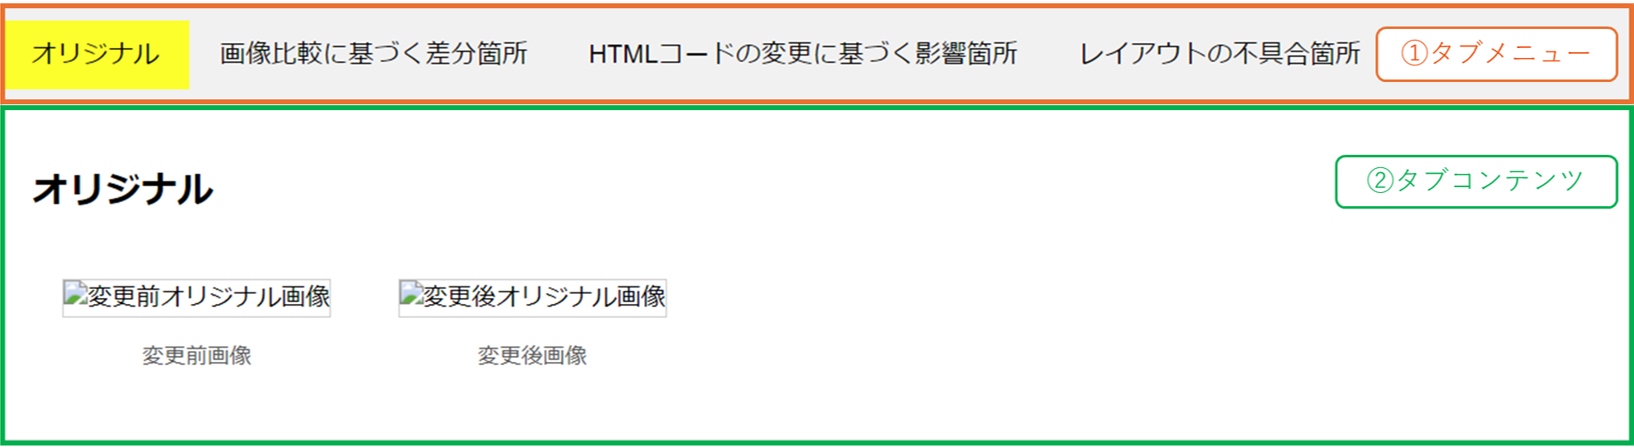
\includegraphics[width=1.0\columnwidth]{image/3_Appearance3.png}
        \caption{\toolName の外観}
        \label{fig: Appearance}
    \end{center}
\end{figure}
\toolName のUIは、以下に示す4つのタブを持つタブメニューと各タブに対応した内容を表示するタブコンテンツからなる。
なお、以下の数字は、図\ref{fig: Appearance}の数字と対応している。
\begin{itemize}
    \item[①] タブメニュー
          \begin{itemize}
              \item オリジナル表示タブ
              \item 画像比較に基づく差分箇所表示タブ
              \item HTMLコードの変更に基づく影響箇所表示タブ
              \item レイアウトの不具合箇所表示タブ
          \end{itemize}
    \item[②] タブコンテンツ
\end{itemize}
\par
\toolName の実行コマンド(\ref{list:command}節を参照)を一度も実行していない場合、
図\ref{fig: Appearance}のように、オリジナル表示タブには、Webページの変更前画像と変更後画像を表示しない。
他の各タブも同様である。
\par
以降、各タブの外観と機能について説明する。

\subsection{オリジナル表示タブ}\label{subsec:original_tab}
オリジナル表示タブを選択すると、Webページの変更前画像と変更後画像を並べて表示する。
オリジナル表示タブを選択した際の\toolName の画面例を、図\ref{fig: Appearance_original_tab}に示す。
\begin{figure}[tp]
    \begin{center}
        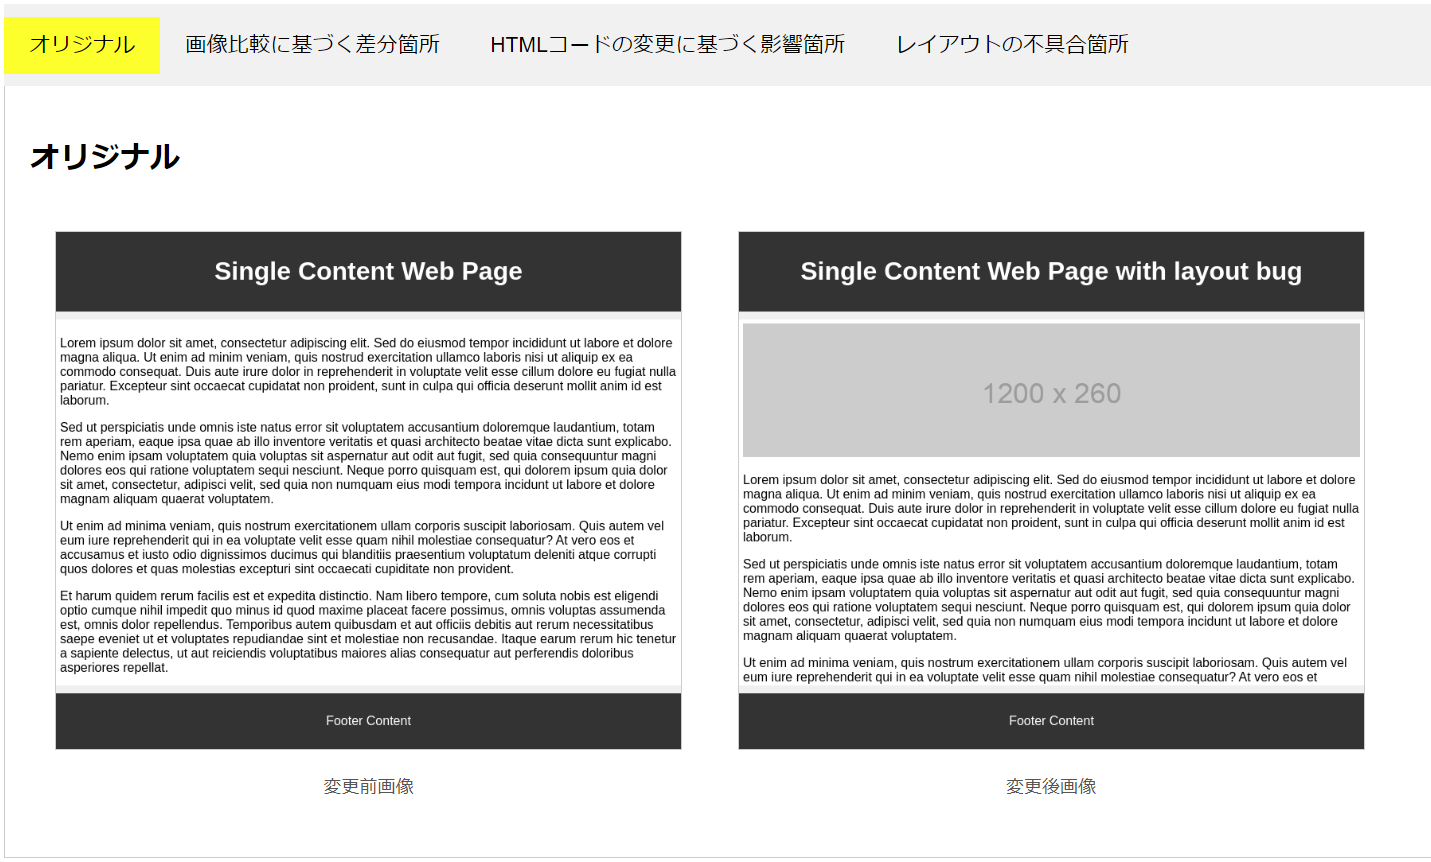
\includegraphics[width=1.0\columnwidth]{image/3_original_tab2.png}
        \caption{オリジナル表示タブを選択した際の\toolName の画面例}
        \label{fig: Appearance_original_tab}
    \end{center}
\end{figure}
なお、\toolName に一番最初にアクセスした時やリロードした時は、初期状態として、オリジナル表示タブを選択する。
このタブでは、Webページの変更前後の画像を目視で確認できる。

\subsection{画像比較に基づく差分箇所表示タブ}\label{subsec:images_tab}
画像比較に基づく差分箇所表示タブを選択すると、画像比較に基づく差分箇所を色付きの枠で囲むことで強調表示した、Webページの変更前画像と変更後画像を並べて表示する。
画像比較に基づく差分箇所表示タブを選択した際の\toolName の画面例を、図\ref{fig: Appearance_images_tab}に示す。
\begin{figure}[tp]
    \begin{center}
        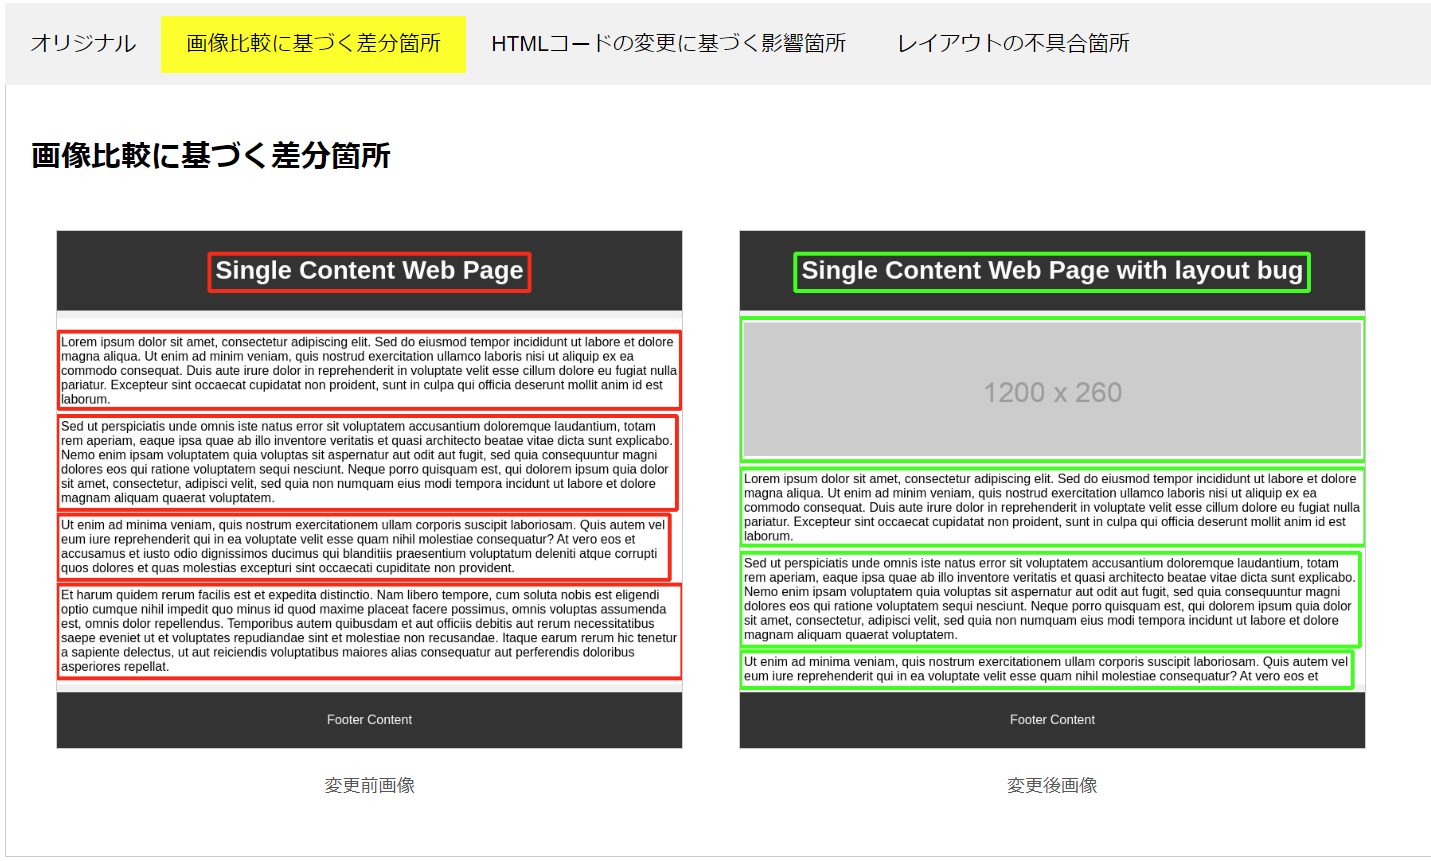
\includegraphics[width=1.0\columnwidth]{image/3_images_tab2.png}
        \caption{画像比較に基づく差分箇所表示タブを選択した際の\toolName の画面例}
        \label{fig: Appearance_images_tab}
    \end{center}
\end{figure}
削除された箇所は変更前画像上に赤枠で囲むことで強調表示し、追加された箇所は変更後画像上に緑枠で囲むことで強調表示する。
このタブでは、変更前後のWebページでレイアウトの変更があった箇所を目視で確認できる。

\subsection{HTMLコードの変更に基づく影響箇所表示タブ}\label{subsec:html_tab}
HTMLコードの変更に基づく影響箇所表示タブを選択すると、HTMLコードの変更に基づく影響箇所を色付きの枠で囲むことで強調表示した、Webページの変更前画像と変更後画像を並べて表示する。
HTMLコードの変更に基づく影響箇所表示タブを選択した際の画面例を、図\ref{fig: Appearance_html_tab}に示す。
\begin{figure}[tp]
    \begin{center}
        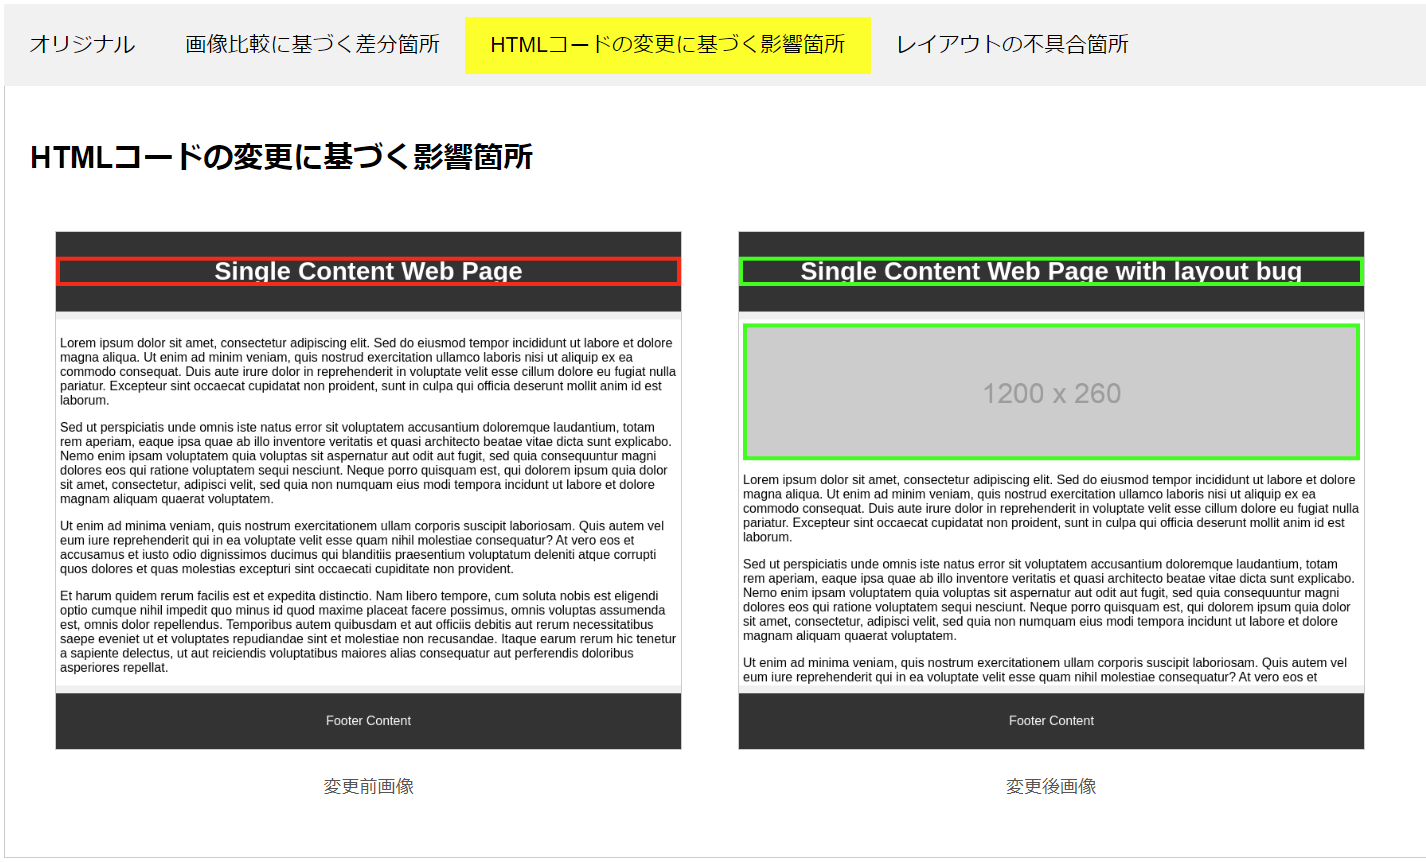
\includegraphics[width=1.0\columnwidth]{image/3_html_tab2.png}
        \caption{HTMLコードの変更に基づく影響箇所表示タブを選択した際の\toolName の画面例}
        \label{fig: Appearance_html_tab}
    \end{center}
\end{figure}
変更前のWebページのHTMLコードにおける影響箇所は変更前画像上に赤枠で囲むことで強調表示し、変更後のWebページのHTMLコードにおける影響箇所は変更後画像上に緑枠で囲むことで強調表示する。
このタブでは、図\ref{fig: Appearance_images_tab}における差分箇所から、開発者が意図して変更した、または意図せず変更してしまったHTMLコードによる影響箇所のみを目視で確認できる。
% このタブでは、変更前後のWebページで開発者が意図した、または意図しないHTMLコードの変更による影響箇所を目視で確認できる。

\subsection{レイアウトの不具合箇所表示タブ}\label{subsec:subeffect_tab}
レイアウトの不具合箇所表示タブを選択すると、検出したレイアウトの不具合箇所を色付きの枠で囲むことで強調表示した、Webページの変更前画像と変更後画像を並べて表示する。
レイアウトの不具合箇所表示タブを選択した際の画面例を、図\ref{fig: Appearance_subEffect_tab}に示す。
\begin{figure}[tp]
    \begin{center}
        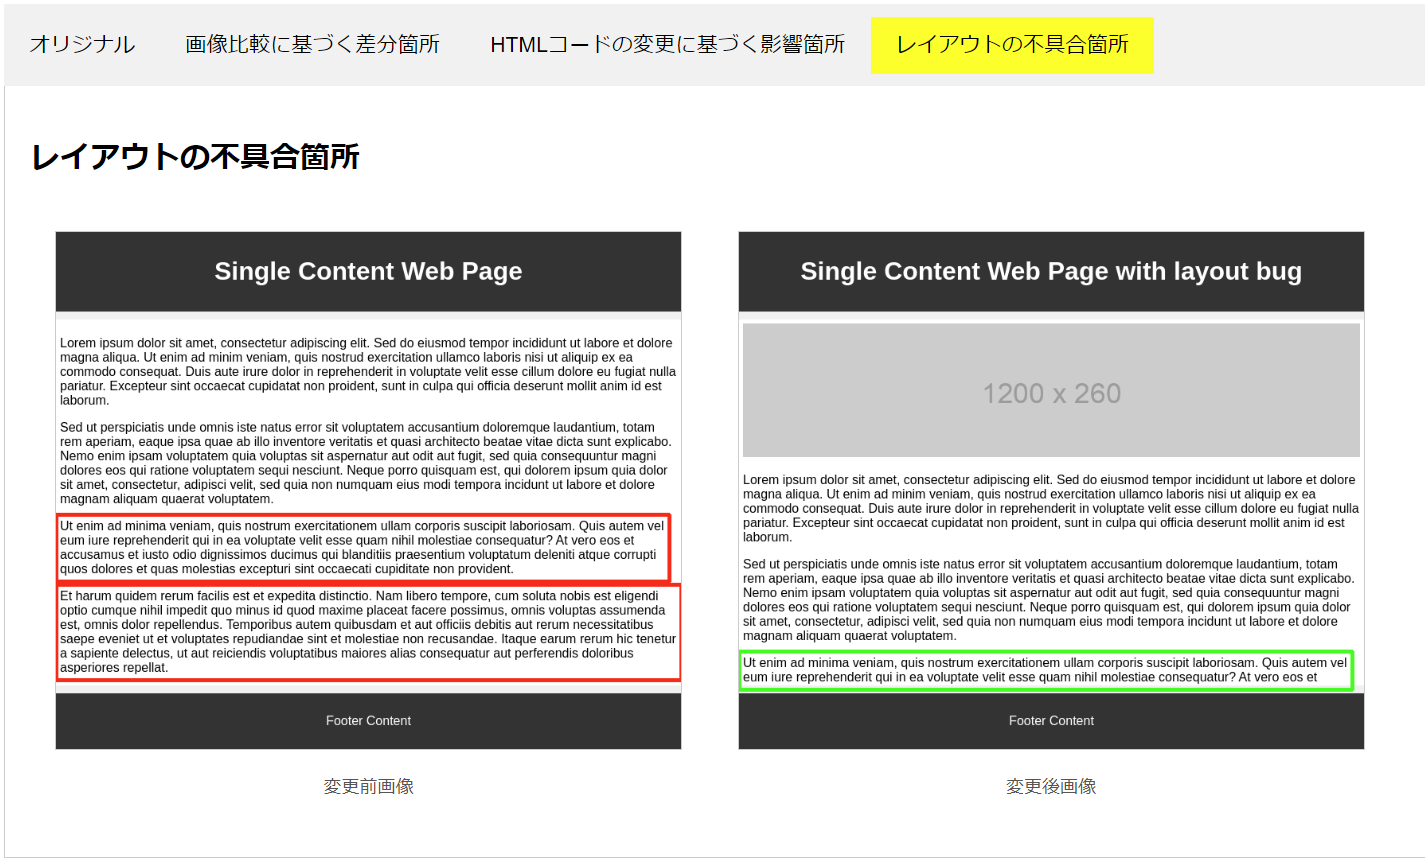
\includegraphics[width=1.0\columnwidth]{image/3_subEffect_tab2.png}
        \caption{レイアウトの不具合箇所表示タブを選択した際の\toolName の画面例}
        \label{fig: Appearance_subEffect_tab}
    \end{center}
\end{figure}
このタブでは、図\ref{fig: Appearance_images_tab}における差分箇所から、レイアウトの不具合箇所のみを目視で確認できる。
図\ref{fig: Appearance_subEffect_tab}の例では、本研究で検出するレイアウトの不具合のうち、画面要素の見切れと画面要素の隠れの2つを見つけることができる。
\par
まず、図\ref{fig: Appearance_subEffect_tab}における画面要素の見切れを、図\ref{fig: out_of_element}に示す。
\begin{figure}[tp]
    \begin{center}
        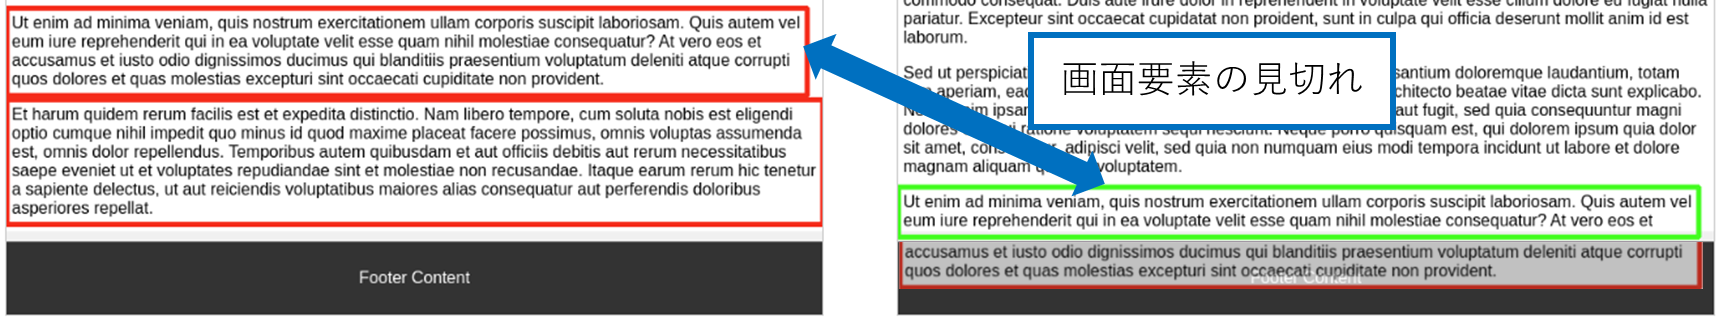
\includegraphics[width=1.0\columnwidth]{image/3_out_of_element2.png}
        \caption{図\ref{fig: Appearance_subEffect_tab}における画面要素の見切れ}
        \label{fig: out_of_element}
    \end{center}
\end{figure}
図\ref{fig: out_of_element}内の青矢印で示した赤枠内と緑枠内のそれぞれのテキストを見比べると、
赤枠内のテキストの上2行目までは緑枠内と同じであるが、赤枠内のテキストの下2行目は緑枠内には存在しない。
また、図\ref{fig: Appearance_html_tab}を見てみると、赤枠内のテキストの下2行目はHTMLコードの変更による影響を受けていないと分かるため、
削除されたわけではない。
よって、Webページの変更後に、テキストの一部がコンテナの境界によって切り取られたことを目視で判断できる。
\par
次に、図\ref{fig: Appearance_subEffect_tab}における画面要素の隠れを、図\ref{fig: hidden_element}に示す。
\begin{figure}[tp]
    \begin{center}
        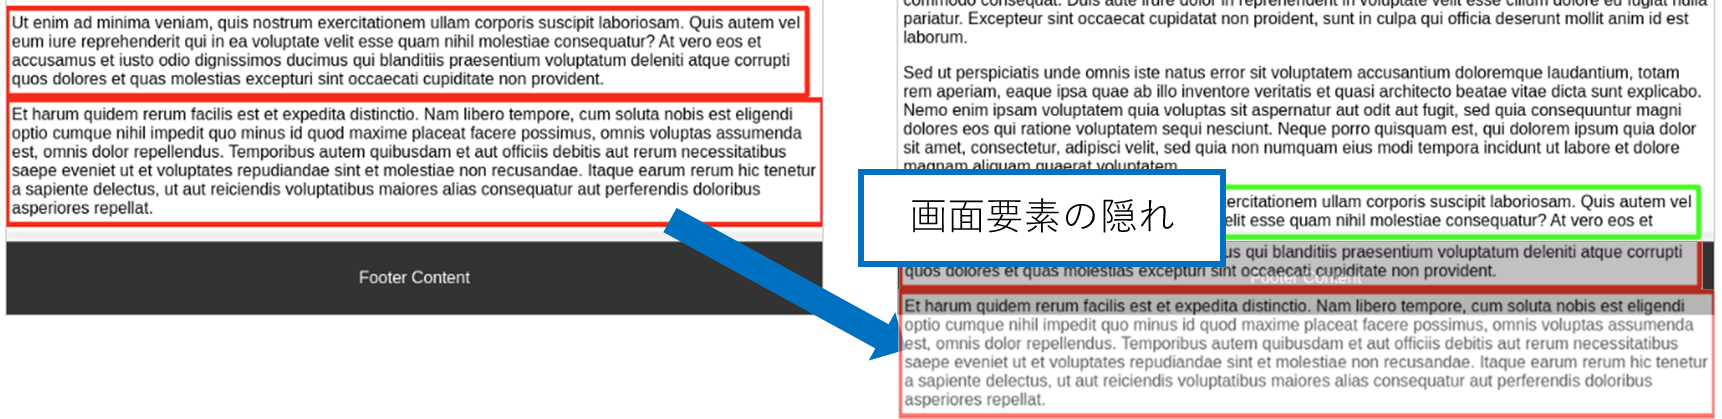
\includegraphics[width=1.0\columnwidth]{image/3_hidden_element2.png}
        \caption{図\ref{fig: Appearance_subEffect_tab}における画面要素の隠れ}
        \label{fig: hidden_element}
    \end{center}
\end{figure}
図\ref{fig: hidden_element}の変更前画像上の一番下にある赤枠内のテキストは、変更後画像上の緑枠内のテキストと一致しない。
また、図\ref{fig: Appearance_html_tab}を見てみると、
一番下の赤枠内のテキストはHTMLコードの変更による影響を受けていないと分かるため、
削除されたわけではない。
よって、図\ref{fig: hidden_element}の青矢印で示すように、
一番下の赤枠内のテキストは、Webページの変更後にコンテナの境界を超えてはみ出した状態になっていると目視で判断できる。
